\documentclass[legalpaper]{article}

\usepackage[english]{babel}
\usepackage[utf8x]{inputenc}
\usepackage{amsmath}
\usepackage{graphicx}
\usepackage[colorinlistoftodos]{todonotes}
\usepackage{geometry}
\usepackage{rotating}
\usepackage{tikz}
\geometry{ hmargin=2cm, vmargin=3cm }
\usepackage[compact]{titlesec}

\title{TP Héritage\\ Conception}
\author{\textbf{Henri HANNETEL - Maria ETEGAN}}
\date{}

\begin{document}
\maketitle

\section*{\large{Introduction}}
\hspace*{\parindent}Le programme \textit{PainTcmd} a pour rôle la gestion de dessins sans interface graphique. L'utilisateur entre des instructions en ligne de commande pour modifier les dessins.\\


\section{Définitions}
\hspace*{\parindent}\textbf{Figure :} L'élément de base du dessin, une figure peut être un cercle, une ligne, une poly-ligne ou un rectangle. \\
\\
\hspace*{\parindent}\textbf{Objet agrégé :} Ensemble constitué de plusieurs figures. \\
\\
\hspace*{\parindent}\textbf{Objet :} Élément graphique du dessin, il peut être une figure ou un objet agrégé. \\


\section{Choix généraux}
\textbf{Ajout d'objets :} \\
\hspace*{\parindent}Les objets sont enregistrés dans le dessin grâce à un dictionnaire dont la clé est calculée à partir du nom de l'objet avec une fonction de hachage (unordered map de la bibliothèque standard de C++11).  Cette solution permet de trouver et d'insérer rapidement une figure. Ce qui est très intéressant car la recherche et l'ajout d'objets sont les opérations les plus utilisées. L'application veille à ce qu'il n'y ait pas deux objets avec le même nom, par contre deux objets peuvent avoir les mêmes coordonnées et être strictement confondus.\\
\\
\textbf{Gestion des figures :} \\
\hspace*{\parindent}Pour que les figures soient manipulées uniformément, elles sont toujours constituées d'une liste de points (deux coordonnées dans le plan). Une figure peut être de quatre type : \textit{cercle}, \textit{ligne}, \textit{poly-ligne} ou \textit{rectangle}. À la différence des autres types, la liste des points du \textit{cercle} est un singleton, le seul point utile étant son centre.\\
\\
\textbf{Gestion des objets agrégés :} \\
\hspace*{\parindent}Un objet agrégé contient la liste des noms des objets qui le composent. Il faut que le dessin contienne au moins deux figures pour pouvoir créer un objet agrégé (hors chargement via un fichier). Un objet agrégé peut contenir un autre objet agrégé.\\
\\
\textbf{Undo et Redo :} \\
\hspace*{\parindent}Les 20 dernières instructions qui ont modifié le dessin sont enregistrées dans une liste. Ainsi on peut déduire la commande inverse et annuler (\textit{undo}) la dernière modification (et les 19 précédentes) à tout moment. On garde toujours la dernière commande en mémoire, afin de pouvoir la refaire (\textit{redo}) si elle a été annulée malencontreusement. L'application ne permet pas d'effectuer plusieurs \textit{redo} à la suite. Après un \testit{CLEAR} le dessin n'est pas supprimé et on garde sa référene en mémoire de manière à ce que son \testit{UNDO} correspondant soit un simple changement de référence. À la suppression d'un objet on garde en mémoire une instance de la figure à supprimer ainsi que des objets agrégés supprimés à cause de la perte de l'objet. Cela permet de recréer tous les objet si l'utilisateur fait un \testit{UNDO}. Une fois les 20 instructions suivantes passées le(s) objets/dessin sont réellement supprimés.\\
\\
\textbf{Suppression d'objets :}\\
\hspace*{\parindent}Lors de la suppression d'un objet on supprime l'objet du dictionnaire puis on parcoure chaque objet agrégé afin de vérifier si il contient l'objet supprimé. Si l'objet supprimé est présent on le supprime et si l'objet agrégé dans lequel ce premier était contenu n'est constitué plus que d'un seul autre objet, on supprime aussi l'objet agrégé. La fonction de suppression est récursive, ce qui permet de supprimer tous les objets agrégés enfant si nécessaire.\\
\\
\textbf{Enregistrement et chargement d'un dessin :} \\
\hspace*{\parindent}L'utilisateur peut à tout moment enregistrer le dessin en cours dans un fichier passé en paramètre. Le logiciel retrouve la commande qui a permis la création de chaque objet et l'enregistre dans le fichier. Cela implique que le dictionnaire soit parcouru entièrement, et comme les éléments ne sont pas ordonnés l'enregistrement se fait dans le désordre, chaque ligne du fichier correspond à une commande. Le chargement d'un dessin se fait en spécifiant le fichier contenant le dessin, les commandes sont ensuite exécutées dans leur ordre d'apparition. Il est possible qu'un objet agrégé soit créé avant les objets qui le constituent. On suppose que l'utilisateur ne crée pas de fichiers à la main, que seule notre application est capable de créer des fichiers, ainsi l'application ne vérifie pas la cohérence des commandes du fichier à charger.\\
\\
\textbf{Remise à zéro :}\\
\hspace*{\parindent}Quand le dessin est remis à zéro via la commande \testit{CLEAR}, on ne le supprime pas tout de suite. Ce n'est qu'une fois la possibilité de faire un \testit{UNDO} écartée que les objets sont réellement supprimés.\\
\\
\textbf{Déplacement d'objet :}\\
\hspace*{\parindent}La fonction de déplacement d'un objet est elle aussi récursive, ce qui permet de déplacer toutes les figures filles d'un objet agrégé. Les figures ne sont déplacées qu'une seule fois même si elles sont contenues plusieurs fois dans l'objet agrégé.\\
\begin{sidewaysfigure}
    \centering
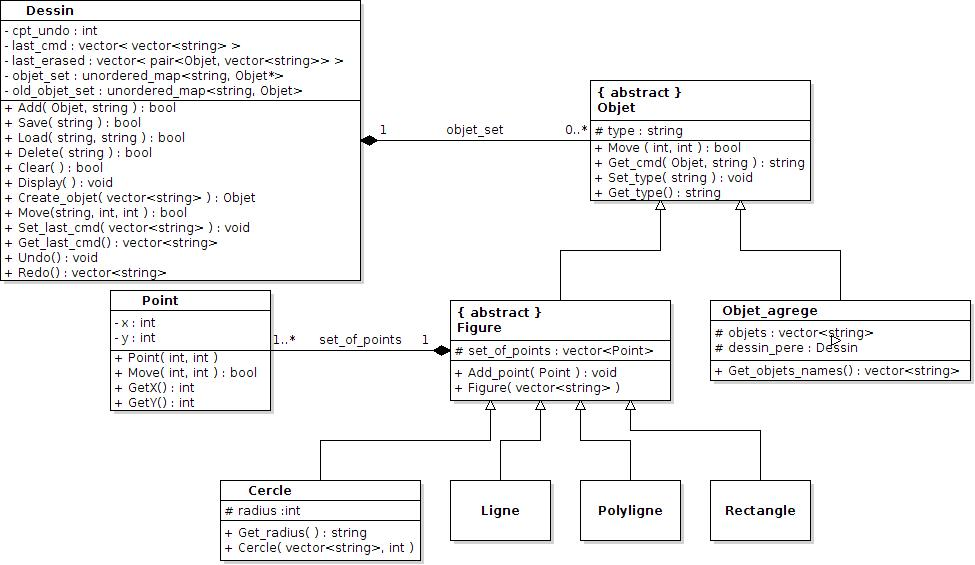
\includegraphics[width=30cm]{Diagramme_objet}
    \caption{Diagramme de classes}
    \label{fig:awesome_image}
\end{sidewaysfigure}
\end{document}